\documentclass[12pt]{article}
\usepackage[utf8]{inputenc}
\usepackage[T1]{fontenc}
\usepackage{titlesec}
\usepackage{listings}
\usepackage{graphicx}
\usepackage{float}
%\usepackage{babel}[it]
% Redefine \ttvar to enable wrapping

\newcommand*\ttvar[1]{\texttt{\expandafter\dottvar\detokenize{#1}\relax}}
\newcommand*\dottvar[1]{\ifx\relax#1\else
  \expandafter\ifx\string.#1\string.\allowbreak\else#1\fi
  \expandafter\dottvar\fi}
\renewcommand{\theparagraph}{\Alph{paragraph}}

\titleformat{\subsubsection}[runin]{\normalfont\bfseries}{\thesubsubsection}{1em}{}[]
\renewcommand{\thesubsubsection}{\arabic{section}.\ifnum\value{subsection}>0{\arabic{subsection}.}\fi\Alph{subsubsection}}

\setcounter{tocdepth}{3}

\title{Peer-Review 1: UML}
\author{Berardinelli, Genovese, Grandi, Haddou\\Gruppo AM21}

\begin{document}

\maketitle
\tableofcontents
\begin{center}
Valutazione del diagramma UML delle classi del gruppo AM30.
\end{center}
\newpage
% -------------
% LATI POSITIVI
% -------------

\section{Lati positivi}
\subsubsection{Incapsulamento e modularità}
I lati positivi del design del modello del gruppo AM30 hanno a che fare sicuramente con una buona separazione delle responsabilità delle classi e dunque con un discreta piattaforma per memorizzare lo stato del gioco.
Il modello segue in linea di massima il principio dell'incapsulamento: i dati sono modificabili e accessibili attraverso interfacce definite che fanno parte della classe che li memorizza come attributi. Ciò promuove la modularità e riduce le dipendenze di una parte dall'altra del modello.

\subsubsection{Chiarezza dell'architettura } La struttura del modello è chiara: le componenti sono ben distinte e hanno la potenzialità di essere effettivamente funzionali se consideriamo singolarmente le loro possibili implementazioni.

\subsubsection{MVC} Il modello rappresentato in diagramma è ben predisposto per il pattern \textit{Model View Controller}.

% -------------
% LATI NEGATIVI
% -------------

\addtocontents{toc}{\setcounter{tocdepth}{2}}
\section{Lati negativi}
Raccogliamo qui una serie di punti, nella speranza che risultino d'aiuto al gruppo in sede di valutazione del progetto.  
\subsection{Criticità del diagramma UML}
\subsubsection{Assenza costruttori delle classi} Poiché sono assenti dal diagramma tutti i costruttori delle classi, non è facile capire quali attributi vengano popolati quando viene istanziato l'oggetto e quali vengano settati a posteriori. Questo talvolta ci ha reso difficile capire quali siano le relazioni tra le classi e dove siano i metodi che gestiscono alcune dinamiche di gioco.
\subsubsection{Assenza di metodi getter e setter} In modo analogo a come descritto nel paragrafo \textbf{A}, l'assenza di \textit{Getter} e \textit{Setter} rende difficile capire come siano state progettate certe dinamiche di gioco. Il \textit{Controller}, eventualmente, si dovrà interfacciare a classi del \textit{Model} i cui attributi sono privati affinchè il player possa giocare il suo turno ed effettuare le sue scelte.
\subsubsection{Posizionamento di alcuni attributi} Alcuni attributi delle classi in diagramma sono posizionati esclusivamente sulle frecce che li uniscono alle classi di cui sono istanza. Comunemente, tutti gli attributi sarebbero da riportare nel box della classe, in modo da riportarne anche la visibilità. Le frecce vanno utilizzate per rappresentare il tipo di relazione fra le classi. Alcuni di questi tipi di associazione sono riportate come \textit{Aggregation} quando in realtà sarebbero \textit{Composition} (vedere \ttvar{CardPair} e i suoi attributi e \ttvar{ComplexObjective} con \ttvar{Layout} eccetera). A nostro parere questo approccio dà poca visione di classe.
\subsubsection{Nits}
\begin{enumerate}
    \item Il \textit{return type} di tutte le funzioni \ttvar{void} è assente.
    \item Il \textit{return type} di \ttvar{Table.drawCard()} e \ttvar{Table.drawObjective()} è assente
    \item La cardinalità di \ttvar{Table.resourceCards}, \ttvar{Table.goldCards}, \ttvar{Table.starterCards} è formalmente 0..* o 0..n
    \item Nei metodi, la sintassi per elencare gli argomenti è talvolta errata: quella corretta è \ttvar{foo(Bar} \ttvar{bar, Car} \ttvar{car): void}
    \item In \ttvar{Table.getDrawableCardsByType()}, se si tratta di un'API generica, manca nei parametri del metodo il numero di carte richiesto da restituire come \textit{Array}.
\end{enumerate}


\subsection{Dinamiche di gioco non gestite}
\subsubsection{Aggiunta del player al gioco} Nel diagramma non è specificato come viene aggiunto l'oggetto \ttvar{Player} a \ttvar{Game.players}, dato che \ttvar{Game.addPlayer()} non prende un \ttvar{Player} come parametro. 
\subsubsection{Gestione del ritmo di gioco} In \ttvar{Game} non sono presenti attributi  che salvino lo stato corrente del gioco come ad esempio il \ttvar{CurrentPlayer}, o il \ttvar{GameState}. In particolare si potrebbe salvare se questo si trovi in uno stato di inizializzazione, se si trovi in attesa che i player si uniscano alla partita, se i player stiano giocando, se si tratti degli ultimi turni o se il gioco sia finito.
\subsubsection{Gestione dell'ultimo turno} Nel diagramma non è specificato come viene gestito l'ultimo turno di gioco. Non sono presenti attributi in \ttvar{Game} che dopo che un player abbia raggiunto un punteggio sufficiente a far terminare la partita e/o le carte siano finite, tiene conto del numero di turni o round rimanenti, prima che il gioco termini effettivamente con \ttvar{Game.endGame()} e dunque siano valutati gli obbiettivi. 
\subsubsection{Token di gioco} Non sono previsti né in \ttvar{Game}, né in \ttvar{Player} attributi che riguardano la serie di \ttvar{Token} assegnabili dal gioco e il colore del \ttvar{Token} scelto dal giocatore.


\subsection{Errori di modellazione}
\subsubsection{Valori non accettabili assegnabili} Da diagramma UML, gli attributi di \ttvar{ComplexObjective.Layout} possono assumere come valori \ttvar{Resource.PEN}, \ttvar{Resource.INKWELL} e \ttvar{Resource.MANUSCRIPT} quando questo in realtà nel gioco non accade.
 Noi suggeriremmo di separarle in due \textit{Enum} differenti.
\subsubsection{Numero di carte in Layout} Le cardinalità di \ttvar{ComplexObjective.Layout} non tornano. Ogni carta ha un massimo di 2 \ttvar{Layout.edges}, perché le carte a destra e sinistra di una carta sulla griglia di gioco sono sfalsate e sono già salvate in \ttvar{Layout.corners}.  
\subsubsection{Angoli "disabilitati"} Non sono modellati gli angoli "disabilitati" delle carte, ovvero gli angoli che non sono \ttvar{Resource.EMPTY} e cui non si può collegare una carta. La cardinalità di \ttvar{Card.cornersFront} dovrebbe essere 0..4, e non 4, per questo motivo. Sebbene esista \ttvar{Table.forbiddenPoints}, il fatto che la carta abbia un angolo disabilitato, per ora, non è salvato da nessuna parte.
\subsubsection{Nits}
\begin{enumerate}
    \item La cardinalità di \ttvar{Player.hand} è di massimo $3$.
\end{enumerate}

\newpage
\subsection{Aree di miglioramento}
Crediamo che per i seguenti aspetti di modellazione esista del margine di miglioramento:
\subsubsection{Riutizzabilità} Gli oggetti collezionabili sono duplicati nelle \textit{Enum} \ttvar{Resource} e \ttvar{Multiplier}, a nostro parere, come anticipiamo in 2.3.A, sarebbe meglio separare Risorse e Oggetti per renderli utilizzabili in modo indipendente utilizzando i generici di Java per utilizzarli in modo più flessibile. 
\subsubsection{Ereditarietà} Concettualmente le \ttvar{Card} non sono tutte uguali. Ad esempio, non tutte le carte \textit{possono} avere una \ttvar{placementCondition}. Ad esempio, la \ttvar{placementCondition} è opzionale per le \textit{GoldCard}, ma una \textit{ResourceCard} non la avrà mai. In quest'ottica, sarebbe meglio, a nostro parere, considerare opzionale un attributo che una certa categoria di carta \textit{può} avere. Si potrebbe gestire meglio questo aspetto con un maggiore uso dell'ereditarietà.
\subsubsection{Opzionalità di alcuni attributi} \ttvar{Resource.EMPTY} non è un vero valore, gli attributi che lo usano potrebbero essere modellati in modo più elegante con un \ttvar{Optional<Resource>}. O meglio, dato che UML è agnostico all'implementazione: \ttvar{Resource[0..1]}. 
\subsubsection{Ridondanza di alcuni riferimenti} Il doppio riferimento a \ttvar{Table} presente in \ttvar{Game} e in \ttvar{Player} è ridondante. La lista di \ttvar{Player} si trova dentro già dentro \ttvar{Game} che ha un unico \ttvar{Table}, si può gestire meglio la situazione con dei \textit{Getter} in \ttvar{Game}, dato che si tratta di funzionalità probabilmente usate dal layer del \textit{Controller}.
\subsubsection{Approccio talvolta poco orientato agli oggetti} Pensiamo che il metodo \ttvar{Table.shuffle()} ne sia un esempio. I mazzi di carte al posto che essere \textit{Array} potrebbero essere rappresentati con un oggetto \ttvar{Deck} che ha un metodo \ttvar{Deck.shuffle()}. Tutto ciò che è effettivamente funzionale da solo potrebbe essere una classe a parte con i suoi metodi.
%%\subsubsection{Doppia gestione delle coordinate} A nostro parere può diventare difficile la gestione del posizionamento delle carte. Perché non usare un \textit{Set} solo di \ttvar{Coordinates} e aggiungere quelle a cui la carta appena posizionata è adiacente e rimuovere quelle che la carta appena posizionata fa diventare \ttvar{Forbidden}? MAYBE TRASFORMARLO IN UN PRO
\subsubsection{Design patterns} Non è riportato in diagramma alcun utilizzo di \textit{creational pattern}. Pensiamo avrebbero la potenzialità di integrarsi bene nel modello se le carte fossero meglio differenziate. Fra i modelli che potrebbero essere utilizzati vi sono il \textit{Factory Pattern} e il \textit{Builder Pattern}.   
\subsubsection{Naming di alcune classi} Ci permettiamo di dare alcuni suggerimenti sul naming di alcune entità o metodi.
\begin{enumerate}
  \item La parola \textit{Points} viene usata sia nei Set di \ttvar{Coordinates} che in \ttvar{Player.points}. Si potrebbe cambiare una delle due per evitare confusione
  \item Il nome di \ttvar{CardPair} non è veramente descrittivo di come è usata la classe. Il nome evoca una coppia di carte giocabili, ma contiene una \ttvar{Card} sola. \\ Vediamo, da come è usato in \ttvar{Player.placeCard()}, che in realtà si tratta di una carta cui è stata scelta la \ttvar{Side} da giocare. Ma allora perché \ttvar{Pair}? Non si capisce, tra l'altro, dove venga chiamato il costruttore, dato che nessun metodo di Player ha come come parametro un \ttvar{Side}.
  %%\item \ttvar{Coordinates}: come mai plurale? Un oggetto dichiarato \ttvar{Coordinates} \ttvar{c} è una coordinata soltanto.
  \item C'è della ripetizione in alcuni nomi di metodi ed attributi. Ad esempio, per \ttvar{Game.endGame()}, \ttvar{Game.startGame()}, \ttvar{Game.gameId} potrebbe essere più elegante usare \ttvar{Game.start()}, \ttvar{Game.end()}, \ttvar{Game.id} eccetera. 
  \item I nomi delle realizzazioni di \ttvar{Objective} non sono molto descrittivi. A nostro parere sarebbe meglio includere la loro natura dentro il nome. Si tratta di obiettivi di conto e di obbiettivi che hanno a che fare con la geometria del \ttvar{Player.playingField}. Simple e Complex non dicono molto. Ma capiamo si tratti veramente di un nitpick. 
\end{enumerate}

\subsection{Perplessità}
\begin{enumerate}
  \item Non è chiaro cosa faccia \ttvar{Supervisor.compute()}. 
  \item Come mai \ttvar{Card.getCorners()} è \textit{Private}?
\end{enumerate}

% ----------------------
% CONFRONTO ARCHITETTURE
% ----------------------
\addtocontents{toc}{\setcounter{tocdepth}{3}}
\newpage
\section{Confronto tra le architetture}

%%Individuate i punti di forza dell’architettura dell’altro gruppo rispetto alla vostra, e quali sono le modifiche che potete fare alla vostra architettur da gestire a per migliorarla.

\subsubsection{Scelte di design sulle responsabilità del modello} L'approccio del gruppo AM30 è sicuramente diverso da quello scelto dal nostro gruppo. Alla base della differenza c'è la \textit{design choice} che riguarda quanto "lavoro" affidare al \textit{controller} che conterrà il \textit{model}, vale a dire il server. 

Come gruppo, abbiamo fatto la scelta di affidare il meno possibile al \textit{controller layer}, offrendo una serie di classi che costruissero un gioco pronto a essere giocato, attraverso i quali metodi lo stato di gioco viene interamente salvato all'interno del modello: lasciando così al server solo la gestione delle comunicazioni con i client. 

L'approccio del gruppo AM30 è diverso nel fatto che sembra che questa serie di metodi e classi, che riguardano la creazione del gioco, dei player, delle carte, poiché non presenti nel diagramma del modello, saranno delegate al controller. 

\subsubsection{Forbidden Points} Abbiamo trovato interessante la doppia gestione delle coordinate in cui è possibile, o meno, piazzare le carte. Come grupppo, avevamo optato per un set solo di coordinate, da aggiornare ogni volta che una carta viene piazzata, scegliendo se aggiungere le posizioni attorno ad essa ad un insieme di cordinate \ttvar{Placeable}. 

Ci rendiamo conto però che avere un set direttamente collegato alle posizioni \textit{forbidden} dovute agli angoli disabilitati ci consente di diminuire il numero di controlli per aggiungere le celle adiacenti a quella in cui avviene il piazzamento a quelle disponibili. 

Contando di piazzare una serie di carte che arriva da due angoli opposti, se una cella è forbidden per la carta che le sta in \ttvar{TOP_LEFT} corner, piazzandone una che sta nel \ttvar{BOTTOM_RIGHT} corner della cella proibita, saprò immediatamente se posso aggiungere la posizione della cella proibita a quelle in cui posso piazzare una carta. Questo controllando se è già presente nel set delle \textit{forbidden}. 

Questo ci risparmia il controllare se alle posizioni libere adiacenti alla carta appena piazzata sono adiacenti carte che hanno l'angolo collegato disabilitato.
Si tratta di approcci in fin dei conti equivalenti ma dal punto di vista grafico, con in mente l'implementazione della \textit{GUI}, ci permette di differenziare l'universo delle celle non raggiungibili da quelle vietate.

\subsubsection{(Nit) GeometricObjective} Fare la review di \ttvar{ComplexObjective.Layout} del modello del gruppo AM30 ci ha fatto realizzare la svista di implementare la struttura dati come una griglia 3x3 di \ttvar{ResourceType}. Si tratta, ovviamente, come nel caso del campo di gioco, di una griglia isometrica e dunque di al massimo  6+1 \ttvar{ResourceType}.

%\subsubsection{TODO: facciamo un BrainStorming}
%\begin{enumerate}
%    \item 
%\end{enumerate}

\section{Appendice}
Alleghiamo in appendice il diagramma presentato dal gruppo AM30.
\begin{figure}[H]
    \begin{center}
        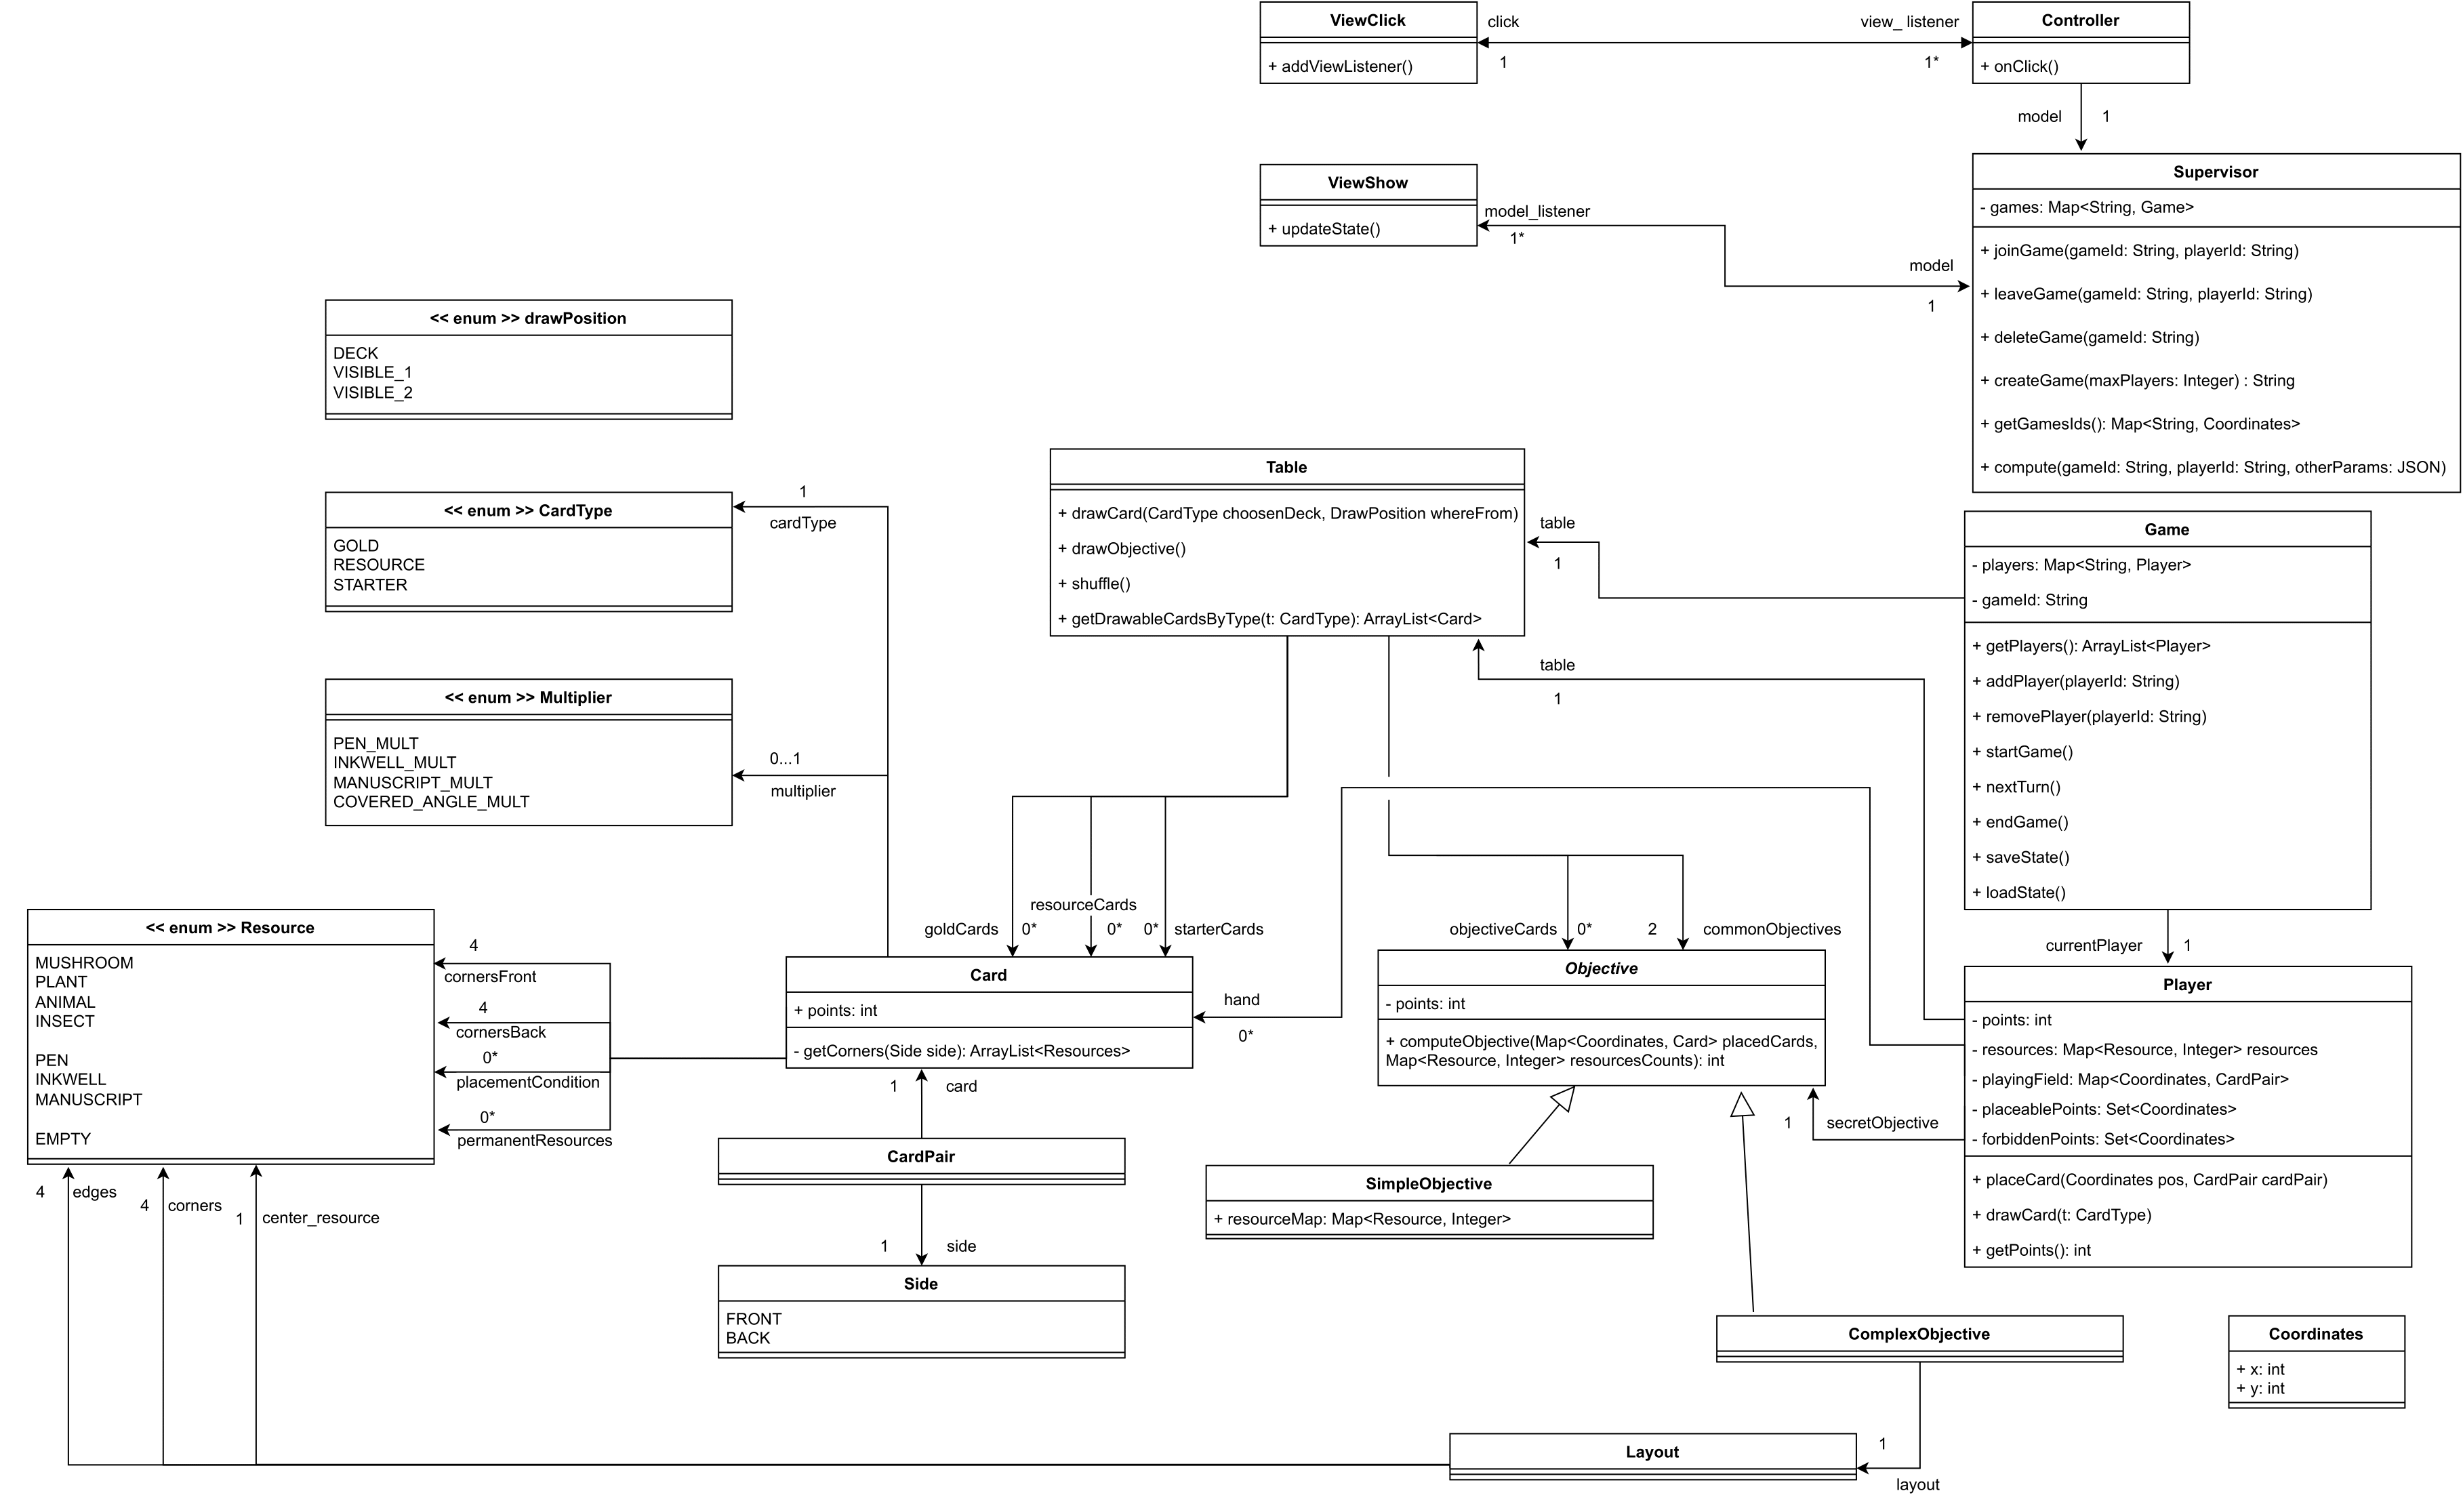
\includegraphics[scale=0.29]{UML_AM30.png}
        \caption{Diagramma UML presentato dal gruppo AM30: model}
    \end{center}
\end{figure}

\end{document}
